\documentclass[12pt,a4paper]{report}
\usepackage[utf8]{inputenc}
\usepackage{amsmath}
\usepackage{amsfonts}
\usepackage{amssymb}
\usepackage{graphicx, neuralnetwork,tikz}
\usepackage{float}
\usetikzlibrary{positioning}
\input defs.tex
%\usepackage[style=numeric]{biblatex}
%\bibliographystyle{alpha}
\usepackage{url}
\graphicspath{ {./figures/} }
\usepackage{cite}


\tikzstyle{process} = [rectangle, minimum width=3cm, minimum height=1cm, text centered, draw=black]
\tikzstyle{arrow} = [thick,->,>=stealth]

\tikzstyle{state}=[shape=circle,draw=blue!30,fill=blue!10]
\tikzstyle{observation}=[shape=rectangle,draw=orange!30,fill=orange!10]
\tikzstyle{lightedge}=[<-, dashed]
\tikzstyle{mainstate}=[state, thick]
\tikzstyle{mainedge}=[<-, thick]
\tikzstyle{block} = [draw,rectangle,thick,minimum height=2em,minimum width=2em]
\tikzstyle{sum} = [draw,circle,inner sep=0mm,minimum size=2mm]
\tikzstyle{connector} = [->,thick]
\tikzstyle{line} = [thick]
\tikzstyle{branch} = [circle,inner sep=0pt,minimum size=1mm,fill=black,draw=black]
\tikzstyle{guide} = []
\tikzstyle{snakeline} = [connector, decorate, decoration={pre length=0.2cm,
                         post length=0.2cm, snake, amplitude=.4mm,
                         segment length=2mm},thick, magenta, ->]




\title{Neural Network Based Decoding over molecular communication Channels}
\author{Peter Hartig}
%Remove this penaltiy if hyphenation is okay. 
%\hyphenpenalty=10000

\begin{document}
\maketitle

\begin{abstract}
Estimation of the probability distribution function characterizing a communication channel is investigated. In this work, pilot symbol sequences are used to train a neural network to estimate unknown channel probability distribution functions. The estimated function is then evaluated using the resulting distribution as a metric for the Viterbi algorithm. In particular, the detection performance is investigated for non-linear channels relevant to the molecular communications domain. A proposal is then made to reduce the complexity of the resulting detection scheme using a clustering of channel states. The neural network based estimation is tested in simulations and shown to be effective in detection for non-linear channels (TODO Finalize for results shown). 
\end{abstract}

\newpage
\tableofcontents
\newpage
\section{Notation}
The following notation is used throughout this work.
$p(x)$ is the probability of an event $x$.
$p(x|y)$ is the conditional probability of $x$ given $y$.
$E[x]$ is the expected value of a random variable $x$.
$\mathcal{N}(0,1)$ denotes Gaussian distribution with mean 0 and variance 1. 

Vectors are denoted by bold font lower-case letters ($\mathbf{x}$) and are assumed column vectors.
The vector $\mathbf{x}_{\mathrm{i}}^{\mathrm{j}}$ denotes a vector containing the elements i through j of $\mathbf{x}$. $|\mathcal{A}|$ denotes the cardinality of the set $\mathcal{A}$.
$\underset{x}{\text{argmin}} \; f(x)$ is the value of variable $x$ which minimizes the function $f(x)$.

\section{Introduction}

The general communication channel is equivalent to a conditional probability distribution function (pdf). The channel pdf $p(\mathbf{x}|\mathbf{y})$ takes into account the (potentially random) channel though which the transmitted information $\mathbf{x}$ passes to reach a receiver as the information $\mathbf{y}$ \cite[Ch.~7]{cover2012elements}. Selecting the most probable transmitted information sequence based on the received information sequence is known as Maximum A-Posteriori Sequence Estimation. In general, sub-optimal solutions to this estimation problem do not require perfect knowledge of the pdf $p(\mathbf{x}|\mathbf{y})$ and may be used when the true $p(\mathbf{x}|\mathbf{y})$ is unknown or impractical to obtain.

\par
Some communication contexts, including wireless, have successfully used "pilot" symbol-streams to estimate the pdf $p(\mathbf{x}|\mathbf{y})$ \cite{van1995channel}. The receiver is informed of a symbol sequence prior to receiving that same sequence sent through the channel. The receiver may then compare the received signal to the known ground truth to obtain information about the channel and estimate the channel $p(\mathbf{x}|\mathbf{y})$.
The use of pilot sequences typically relies on some pre-selected channel model with parameters determined using the pilot sequence. For example, if the channel is assumed to be a noiseless LTI system, the pilot sequences may be used to find the exact impulse response of the channel (CITE or reference to below). In some cases, however, a precise channel model may not be available. In this work, we investigate the parameterization of a very general form of $p(\mathbf{x}|\mathbf{y})$ using a neural network based channel model. In previous work, neural network based estimation of the channel has shown to be an effective method for detection with incomplete channel information for linear, time-invariant channels \cite{shlezinger2019viterbinet} \cite{shlezinger2020datadriven}.
 Extending on this, we look to estimate $p(\mathbf{x}|\mathbf{y})$ for channels in the molecular communication domain.
 We also look to exploit any redundancy in the pdf $p(\mathbf{x}|\mathbf{y})$ in order to reduce the complexity of the resulting detection algorithm. (TODO Remove if not working)
\par
Molecular communication channels can be difficult to characterize due to non-linearity, randomness and dependence upon the transmitted information. As a result molecular communication channels are good candidates for testing this estimation technique. For a thorough review and mathematical formulation of molecular communication channels and their applications see \cite{jamali2019channel}. 
\par

(Discuss a rate/robustness trade-off in the model?)
% As no information is communicated from transmitter to receiver in this process, the use pilot sequences is not feasible for all channels. If the estimate of $p(\mathbf{x}|\mathbf{y})$ derived from pilot symbols does not offer sufficient, relevant channel information when subsequent symbols with real information are transmitted, this will not offer any benefit. Additionally, the resource overhead of sending symbols without information may not be tolerated in some contexts.



\par

\section{System Model}

A system model is now developed as a consistent communication framework to be used in the remainder.
\par
We consider a point to point communication system as in Figure \ref{fig:model} with a transmitter sending a sequence of information $\mathbf{x}$ over a channel. At the receiver, the sequence  $\mathbf{y}$ is detected. 
The elements of $\mathbf{x}$ are chosen from a finite symbol alphabet $\mathcal{A}$ such that $x[\text{k}] \in \mathcal{A}$.

\begin{figure}[H]
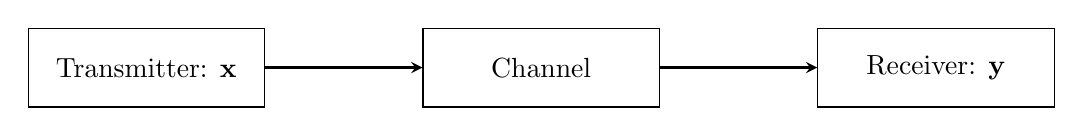
\begin{tikzpicture}[node distance=2cm]
\node (transmitter) [process] {Transmitter: $\mathbf{x}$};
\node (channel) [process, right = of transmitter] {Channel};
\node (receiver) [process, right = of channel] {Receiver: $\mathbf{y}$};
\draw [arrow] (transmitter) -- (channel);
\draw [arrow] (channel) -- (receiver);
\end{tikzpicture}
\caption{The point to point communication system.}
\label{fig:model}
\end{figure}

The components of the vector $\mathbf{y}$ are described by 
\begin{equation*}
y[\text{k}] = f_{\text{k}}(\mathbf{x}) + n[\text{k}],
\end{equation*}
with independent $n[\text{k}]\sim \mathcal{N}(0,1).$
Allowing for $f_{\text{k}}()$ to be a general and potentially random function, each received symbol $y[\text{k}]$ is a function of all input information $\mathbf{x}$.

By assuming all $n[\text{k}]$ to be independent, an orthogonal filtering of the modulated information $\mathbf{x}$ at the receiver is implied. As a result the signal to noise ratio (SNR) is defined using ... (Square root nyquist can be assumed for continuous time receiver filter)
TODO discuss modulation and filtering assumptions that are made. 

Is it okay for the SNR to be defined as the energy at the receiver and not at the transmitter?

\begin{equation*}
\text{SNR} = \frac{E\{|x[\text{k}]|^2\}}{\sigma^2}.
\end{equation*}
\par

Now describe specific cases of the channel function. 

In the first communication channel $f_{\text{k}}(\mathbf{x}) + n[\text{k}]$ considered each $y[\text{k}]$ is a causal, linear, and time-invariant (LTI) combination of the transmitted sequence $[x[\text{k}], x[\text{k}-1]... x[\text{K}-\text{L}+1]]$ weighted by coefficients $[a[0], a[1].. . [\text{L}-1]]$. 
\begin{equation*}
y[k] = \sum_{\mathrm{\text{l}=0}}^{\mathrm{\text{L}-1}} a[\text{l}]x[\text{k}-\text{l}].
\end{equation*}

\par 
We also consider the case in which the received output from an arbitrary communication channel is quantized giving
\begin{equation*}
y[\text{k}] = Q(f_{\text{k}}(\mathbf{x}) + n[\text{k}])
\end{equation*}
 with $Q()$ is defined by 
\[Q(x) = 
\begin{cases}
floor(x)\\
\text{upper saturation level}\\
\text{lower saturation level}
\begin{cases}
]\ 
 
 
\section{Background}
The following section first introduces the optimization problem used in the remainder of this work. An efficient implementation for solving the optimization problem is then introduced. With this foundation in place, the data-driven, neural network based model is then incorporated into the optimization algorithm. 
Extending on the neural network based detector, a method to further reduce the algorithm complexity is then considered. Lastly, a linear equalizer is derived to be used as a reference in the simulation results. 
\subsection{MLSE and the Viterbi Algorithm}

Selecting the most probable transmitted information sequence based on the received information sequence is known as Maximum A-Posteriori Sequence Estimation and is formalized as
\begin{equation*}
\underset{x\in\mathcal{A}^N}{\text{argmax}} \; p(\mathbf{x}|\mathbf{y}),
\end{equation*} 

with $\mathcal{A}^N$ being the set of possible transmitted sequences $\mathbf{x}$.
Using Bayes' theorem, we can equivalently use 
\begin{equation*}
p(\mathbf{x}|\mathbf{y}) = 
\frac
{p(\mathbf{y}|\mathbf{x})p(\mathbf{x})}
{p(\mathbf{y})}.
\end{equation*}
If all $x\in\mathcal{A}^N$ are selected with equal probability, as is commonly assumed to maximize information entropy for finite $|\mathcal{A}|$, the term $p(\mathbf{x})$ can be removed without effect. Similarly, because the term $p(\mathbf{y})$ is independent of $\mathbf{x}$ it can also be removed without effect. The resulting optimization problem
\begin{equation}\label{opt_problem}
\underset{x\in\mathcal{A}^N}{\text{argmax}}\; p(\mathbf{y}|\mathbf{x}),
\end{equation}
known as Maximum Likelihood Sequence Estimation (MLSE), will be used in the remainder.
Noting that the size of the search space $|\mathcal{A}^N|$ grows exponentially in $N$, the number of transmitted symbols, a method for reducing the search complexity is introduced. 
\par
Consider the communication channel for which each $y[\text{k}]$ is a causal, linear, and time-invariant (LTI) combination of the transmitted sequence $[x[\text{k}], x[\text{k}-1]... x[\text{K}-\text{L}+1]]$ weighted by coefficients $[a[0], a[1].. . [\text{L}-1]]$. 
\begin{equation*}
y[k] = \sum_{\mathrm{\text{l}=0}}^{\mathrm{\text{L}-1}} a[\text{l}]x[\text{k}-\text{l}].
\end{equation*}
For this channel,
\begin{equation*}
\underset{\mathbf{x}\in\mathcal{A}^N}{\text{argmax}} \; p(\mathbf{y}|\mathbf{x})=
\underset{\mathbf{x}\in\mathcal{A}^N}{\text{argmin}} \; \sum_{\mathrm{i=1}}^{\mathrm{N}} -\text{log}(p(y_{\mathrm{i}}|\mathbf{x}_{\mathrm{i-L+1}}^{\mathrm{i}}) ),
\end{equation*}
in which individual terms of the sum are statistically independent. This channel can be equivalently represented by 
the set of states $\{s_1, s_2,.. s_{\text{L}}\}$ with each state $s_{\text{l}}$ representing one of the possible $\mathbf{x}_{\mathrm{i-L+1}}^{\mathrm{i}} \in \mathcal{A}^{\text{L}}$. The entire sequence $[y[1]... y[\text{N}]]$ is then
  represented by repeating these states N times with all states $s_{\text{i}}^{\text{k}}$ in time k connected to all states $s_{\text{j}}^{\text{k+1}}$ in time k$+1$
%  It is important to note that for a specific time point $y[\text{k}]$,
%   each state $s_{\text{l}}$ implies a specific transmit symbol $x[k]$ in that time point. Edges between states in k and k$+1$ are made only if $x[\text{k}]= x[\text{k-1}]$ for the $\mathbf{x}_{\mathrm{i-L+1}}^{\mathrm{i}}$ represented by $s_{\text{i}}^{\text{k}}$ and $s_{\text{j}}^{\text{k+1}}$. 
   by an edge weighted with
\begin{equation*}
-\text{log}(p(s_{\text{l}}^{\text{k+1}}|s_{\text{j}}^{\text{k}})p(y[\text{k}+1]|s_{\text{l}}^{\text{k+1}})).
\end{equation*}   
This is illustrated in the following example. 
   \par
   Consider the communication system with $\mathcal{A}=\{0, 1\}$ and received symbols 
   \begin{equation*}
y[\text{k}] =  a[\text{0}]x[\text{k}] + a[\text{1}]x[\text{k}-1] + n[\text{k}],
\end{equation*}
with $n[\text{k}] \sim \mathcal{N}(0,1)$.
The resulting state graph (or trellis) is depicted in Figure \ref{fig:trellis}. 
Again assuming equiprobable 
$\mathbf{x}_{\mathrm{i-L+1}}^{\mathrm{i}} \in \mathcal{A}^{\text{L}}$, the value of $p(s_{\text{j}}^{\text{k+1}}|s_{\text{i}}^{\text{k}})$ for connected states $s_{\text{j}}^{\text{k+1}}$ and $s_{\text{j}}^{\text{k}}$ is either some constant c ($0<$c$\leq1$) or 0, depending on whether or not $x[\text{k}]= x[\text{k-1}]$ for the $\mathbf{x}_{\mathrm{i-L+1}}^{\mathrm{i}}$ represented by $s_{\text{j}}^{\text{k+1}}$ and $s_{\text{j}}^{\text{k}}$(Too confusing). For clarity all edges for which $p(s_{\text{j}}^{\text{k+1}}|s_{\text{i}}^{\text{k}})=0$ have been removed. Therefore the shown edges into state $s_{\text{i}}^{\text{k+1}}$ are weighted by
$-\text{log}(p(y[\text{k}+1]|s_{\text{j}}^{\text{k+1}})$. The solution to problem \ref{opt_problem} corresponds to the minimum cost path through all N sets of states which can be found using the Viterib algorithm. 
\\

    \noindent\rule[16pt]{\textwidth}{0.6pt}
	Viterbi Algorithm: (TODO: Decide if this is clear enough)

    \noindent\rule[10pt]{\textwidth}{0.4pt}
    {\footnotesize
    \begin{tabbing}
        {\bf given} $p(y_{\mathrm{i}}|x_{\mathrm{i-L+1}}^{\mathrm{i}}) \; \forall  \;i \in {1..N}$. \\*[\smallskipamount]
        {\bf for $i = 1...N $} \\
         \qquad \= {\bf for each state $s \in \mathcal{A}_{\mathrm{i-L+1}}^{\mathrm{i}}$}\\
        \qquad \qquad \= 1.\ Let $\text{cost}_{s}^{\text{i}} = -\text{log}(p(y_{\mathrm{i}}|x_{\mathrm{i-L+1}}^{\mathrm{i}})) + \underset{s}{\text{min}} \{\text{incoming costs}_{s}^{\text{i-1}}\}$ \\
%        \> 2.\ {\bf break if} $f(z) \leq \hat{f}_{\lambda}(z, x^{k})$. \\
%        \> 3.\ Update $\lambda := \beta \lambda$. \\*[\smallskipamount]
        {\bf return} detected transmission $\hat{\mathbf{x}}$ corresponding to trellis path of $\underset{s}{\text{argmin}} \; \text{cost}_{s}^N $
    \end{tabbing}}
    \noindent\rule[10pt]{\textwidth}{0.4pt}



\begin{figure}[H]
\begin{center}
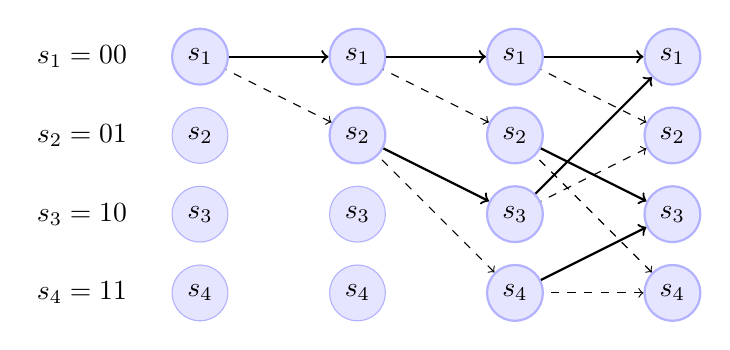
\begin{tikzpicture}[]
% 1st column
\node               at (-1.5,5) {$s_1=00$};
\node               at (-1.5,4) {$s_2=01$};
\node               at (-1.5,3) {$s_3=10$};
\node               at (-1.5,2) {$s_4=11$};
\node[mainstate] (s1_1) at (0,5) {$s_1$};
\node[state] (s2_1) at (0,4) {$s_2$};
\node[state] (s3_1) at (0,3) {$s_3$};
\node[state] (s4_1) at (0,2) {$s_4$};
%\node at (0,1) {Node1};
% 2nd column
\node[mainstate] (s1_2) at (2,5) {$s_1$}
    edge[mainedge] (s1_1);
\node[mainstate] (s2_2) at (2,4) {$s_2$}
     edge[lightedge] (s1_1);

\node[state] (s3_2) at (2,3) {$s_3$};

\node[state] (s4_2) at (2,2) {$s_4$};

%\node at (2,1) {Node2};
% 3rd column
%\node               at (4,6) {$t=2$};
\node[mainstate] (s1_3) at (4,5) {$s_1$}
    edge[mainedge]  (s1_2);

\node[mainstate] (s2_3) at (4,4) {$s_2$}
    edge[lightedge] (s1_2);

\node[mainstate] (s3_3) at (4,3) {$s_3$}
    edge[mainedge] (s2_2);    
\node[mainstate] (s4_3) at (4,2) {$s_4$}
    edge[lightedge] (s2_2);
%\node at (4,1) {Node3};
% 4th column
%\node               at (6,6) {$t=3$};
\node[mainstate] (s1_4) at (6,5) {$s_1$}
    edge[mainedge]  (s1_3)
    edge[mainedge]  (s3_3);
\node[mainstate] (s2_4) at (6,4) {$s_2$}
    edge[lightedge] (s1_3)
    edge[lightedge] (s3_3);
\node[mainstate] (s3_4) at (6,3) {$s_3$}
    edge[mainedge] (s2_3)
    edge[mainedge] (s4_3);
\node[mainstate] (s4_4) at (6,2) {$s_4$}
    edge[lightedge] (s2_3)
    edge[lightedge] (s4_3);
%\node at (6,1) {Node4};

\end{tikzpicture}
	\end{center}
	\caption{MLSE decoding for $\mathcal{A}=\{0,1\}$ and $L=2$. Each state $s_1 ... \; s_4$ represents a possible
	$\mathbf{x}_{\mathrm{i-L+1}}$.}
	\label{fig:trellis}
\end{figure}


The Viterbi Algorithm  computes the MLSE for any finite state, causal channels (REMOVE?).

Note that the Viterbi algorithm is \emph{linearly} complex in the length of the transmitted sequence $\mathbf{x}$ ($N$ in the algorithm above) but \emph{exponentially} complex in the number of channel states ($|\mathcal{A}_{\mathrm{i-L+1}}^{\mathrm{i}}|$ for the LTI channel above). 
\par
In the remainder of this work, we consider the case in which the  channel state is determined entirely by $\mathbf{x}_{\mathrm{i-L+1}}^{\mathrm{i}}$, as was the case for the LTI channel. By adding additional states, this same approach can be extended to channel with random components independent of the input $\mathbf{x}_{\mathrm{i-L+1}}^{\mathrm{i}}$.

(Add final limit on this noting that this only works if the randomness can be represented by a markov chain??)

\subsection{ViterbiNet}
(Nice area to describe how in this noiseless, time-invariant case we only need L samples to perfectly estimate channel and how this wouldn't be possible for the neural network)
\par

Despite the complexity reduction of the Viterbi Algorithm for MLSE, weighting the edges of the graph requires knowledge of the channel probability distribution $p(y_{\mathrm{i}}|s_{\mathrm{k}})$. Rather than estimate this function directly, we use Bayes' theorem and instead estimate the individual terms of
\begin{equation*}
p(y[\mathrm{i}]|s_{\text{i}}^{\text{k}}) = 
\frac
{p(s_{\text{i}}^{\text{k}}|y[\mathrm{i}])p(y[\mathrm{i}])}
{p(s_{\text{i}}^{\text{k}})}.
\end{equation*}

\begin{itemize}
\item $p(s_{\text{i}}^{\text{k}}|y_{\mathrm{i}})$: 
For a channel with finite states $\{s_1, s_2,.. s_{\text{L}}\}$, this probability mass function can be estimated using a neural network for classification. Each training data pair includes a single received pilot symbol $y[\text{k}]$ with the known transmit symbols (channel state) 
$s_{\text{i}}^{\text{k}} \sim \mathbf{x}_{\mathrm{\text{k}-\text{L}+1}}^{\mathrm{\text{k}}}$. By using using a network architecture with a number of outputs corresponding to the number of channel states, the trained network will take input $y[\text{k}]$ and output the desired $p(s_{\text{i}}^{\text{k}}|y_{\mathrm{i}})$ for all $s_{\mathrm{k}} \in \textit{\cal{S}}$. Figure \ref{nn} depicts the neural network for a channel with four states. The shown network has a total of 20 parameters to be optimized during training. For a detailed review of classification using neural networks, see \cite[Ch.~5]{Goodfellow-et-al-2016}
(TODO: for the chosen cost function is this is the ML estimator for the model?)(TODO include cost function)
	\begin{figure}[H]
	\centering
		\begin{neuralnetwork}[height=4, nodespacing=10mm, layerspacing=15mm]
		\newcommand{\x}[2]{$y_#2$}
		\newcommand{\y}[2]{$s_#2$}
		\newcommand{\hfirst}[2]{\small $h^{(1)}_#2$}
		\newcommand{\hsecond}[2]{\small $h^{(2)}_#2$}
		\newcommand{\hthird}[2]{\small $h^{(3)}_#2$}
		\newcommand{\hfourth}[2]{\small $h^{(4)}_#2$}
		\inputlayer[count=1, bias=false, title=Received\\, text=\x]
		\hiddenlayer[count=2, bias=false, title=\\, text=\hthird] \linklayers
		\hiddenlayer[count=3, bias=false, title=\\, text=\hfourth] \linklayers
		\outputlayer[count=4, title=States\\, text=\y] \linklayers
	    \end{neuralnetwork}
	    	  	  \caption{A neural network architecture for classification of received symbols into four channel states.}
\label{nn}
	\end{figure}

\item $p(y[\mathrm{i}]) = \sum_{s_{\mathrm{k}} \in \textit{$\mathcal{S}$}}p(s_{\mathrm{k}},y[\mathrm{i}])$: This term is found by marginalizing the joint probability of channel state $s_{\mathrm{k}}$ and received signal $y[\mathrm{i}]$ over all channel states $\mathcal{S}$. As $p(y[\mathrm{i}])$ is constant over all states in a given step of the Viterbi algorithm, it may be interpreted as a weighting factor for the cost of received symbol $y[\mathrm{i}]$ relative to other symbols $y[\mathrm{j}], \; j\neq i$. For example, if $y[\mathrm{i}]$ is received under improbable noise and channel state, this term would reduce the overall impact of $y[\mathrm{i}]$ on the final path chosen through the graph. In the case of equiprobable channel states without receiver noise $p(y[\mathrm{i}])$ would be constant and have no impact on the path.
\par
This probability distribution function can be estimated using a so-called mixture-model. This requires pre-selecting the number of considered channel states and a parameterized model for receiver noise. The Expectation Maximization algorithm, detailed in \cite{ng2000cs229}, along with a set of channel output can be used to optimize this model. Unlike parameterizing the neural network this algorithm does not require labeled data. 
 (Figure \ref{fig:mm})
(TODO decide whether or not to swap state and transmit sequence)
%\\
%
%    \noindent\rule[16pt]{\textwidth}{0.6pt}
%	Expectation Maximization Algorithm for Gaussian Mixture Model: (TODO Discuss how much derivation is needed here)
%
%    \noindent\rule[10pt]{\textwidth}{0.4pt}
%    {\footnotesize
%    \begin{tabbing}
%        {\bf given} $p(y_{\mathrm{i}}|x_{\mathrm{i-L+1}}^{\mathrm{i}}) \; \forall i \in {1..N}$ . \\*[\smallskipamount]
%        {\bf for $i = 1..N $} \\
%         \qquad \= {\bf for each state $s$ at time $i$}\\
%        \qquad \qquad \= 1.\ Let $\textit{survivor cost}_{s}  += \text{min}\{\text{incoming transition costs}\}$ \\
%%        \> 2.\ {\bf break if} $f(z) \leq \hat{f}_{\lambda}(z, x^{k})$. \\
%%        \> 3.\ Update $\lambda := \beta \lambda$. \\*[\smallskipamount]
%        {\bf return} Symbols corresponding to path of $\underset{s}{\text{argmin}} \; \textit{survivor cost}_{s} $
%    \end{tabbing}}
%    \noindent\rule[10pt]{\textwidth}{0.4pt}


%picture of MM
%	\includegraphics[width=\textwidth,height = 7cm]{results/quant_standard}

\begin{figure}[H]
\centering
	\includegraphics[width=\textwidth,height = 10cm]{system_model/mm}
	  	  \caption{A mixture of complex, Gaussian sources that can be estimate using the Expectation Maximization algorithm}
	  \label{fig:mm}
\end{figure}

\item $p(s_{\text{k}})$: For the case in which each channel state is equiprobable, such as when $s_{\text{k}}$ corresponds to $\mathbf{x}_{\mathrm{i-L+1}}^{\mathrm{i}}\in \mathcal{A}_{\mathrm{i-L+1}}^{\mathrm{i}}$, this term will not influence the final path and can be neglected.

\end{itemize}

Combining these terms and their impact on the original $p(y[\mathrm{i}]|s_{\text{i}}^{\text{k}})$, each edge weight used in the Viterbi algorithm essentially gives the probability of arriving at a state $p(s_{\text{k}})$ conditioned on the previous state $p(s_{\text{k-1}})$ and the received signal $y[\mathrm{k}]$ weighted by the probability of receiving $y[\mathrm{k}]$ based on the channel and noise. 
We investigate how a channel might be represented using the minimum number of states.

\subsection{A Reduced State ViterbiNet}
While the Viterbi Algorithm complexity scales exponentially in the number of states possible in each step of the algorithm, in some cases this complexity can be reduced without significant loss of detection performance. 
In particular, this is possible if the system is such that some channel states are redundant. The following, relevant example with state redundancy is posed and one potential method of reducing the number of states is then considered. 

Consider a received signal from an LTI communication channel
\begin{equation*}
y[k] = \sum_{\mathrm{l=1}}^{\mathrm{L}} a[l]x[k-l] + n[k], \; n[k]  \sim \mathcal{N}(0,1)
\end{equation*}

with  $\mathcal{A}=\{-1, 1\}$ and $n[k]  \sim \mathcal{N}(0,1)$.  

For $\mathbf{a} = [a[1]...a[5]]=[1, 0, .2, .2, .4]$ ($\|\mathbf{a}\|^2_2 = 1$), the received signal is shown in Figure \ref{fig:redundant_channel}. Desipite having channel memory L $=5$, there are fewer than the potential $|\mathcal{A}_{\mathrm{i-L+1}}^{\mathrm{i}}| =2^5$ clusters of received signals. This is due to the redundancy in the channel.  As one of the channel taps is 0, this will have no impact on the output and thus 16 of the potential 32 states are removed. Further, as there are two taps of value 0.2 and $\mathcal{A}=\{-1, 1\}$, when $[x[k-2],x[k-3]] = [-1,1]$ and $[x[k-2],x[k-3]] = [1,-1]$ these map to the same state. 

%\begin{figure}[H]
%\centering
%	\includegraphics[width=10cm,height = 10cm]{system_model/channel_output}
%	  \label{fig:redundant_channel}
%	  	  \caption{LTI channel with state redundancy with high SNR}
%\end{figure}


\par
Pre-filtering section. Regardless, this sort of pre-filtering will require some sort of channel estimate which will require some model. 
Can also mention that this might introduce latency into the system unlike the design used here. 
\par

An alternative, data-driven approach to exploiting state redundancy is to cluster the original states into a set of $k<|\mathcal{A}|$ clusters using training data. The K-Means algorithm is proposed as one such clustering method.
\\

    \noindent\rule[16pt]{\textwidth}{0.6pt}
K-Means Clustering Algorithm: A method for unsupervised classification

    \noindent\rule[10pt]{\textwidth}{0.4pt}
    {\footnotesize
    \begin{tabbing}
    {\bf given} initial location $L_c, \forall \;c  \in \{1..K\}$ of K centroids.\\
        {\textbf{for} Number of Iterations}.\\
         \qquad \= {\bf for each training data point $x_{\mathrm{i}}, \;\mathrm{i}  \in \{1..N\}$}\\
        \qquad \qquad \= 1.\ Label $x_i$ with the index c of the closest centroid using $\|x_{\mathrm{i}}- \text{L}_c\|^2_2$. \\
        \qquad \= {\bf for centroid $L_c, \forall \;c  \in \{1..K\}$}\\
                \qquad \qquad \= 1.\ Move $L_{\mathrm{c}}$ to the average location of all training points with label .c\\


%        \> 2.\ {\bf break if} $f(z) \leq \hat{f}_{\lambda}(z, x^{k})$. \\
%        \> 3.\ Update $\lambda := \beta \lambda$. \\*[\smallskipamount]
        {\bf return} Centroid locations.
    \end{tabbing}}
    \noindent\rule[10pt]{\textwidth}{0.4pt}
    

\par
An important implementation consideration for this clustering approach is now discussed. If the channel has memory $\text{L}>1$, at least some of the channels states represent different channel inputs as described previously. If states with contradicting transmission memory are clustered during the state reduction the choice for the transmitted symbol is unclear. To accommodate this scenario, a majority rule decision is made, based on the final state path chosen by the Viterbi algorithm. During the clustering, the fraction of training samples from the original states labeled in each reduced state are recorded to give the likelihood of each symbol in the state memory. After finding the lowest cost path through the trellis, the probability of a symbol for each time index is found and the most likely is chosen. Note that this operation is \emph{not} exponentially complex in the memory length of the channel and is only performed once before deploying this detector scheme. (TODO still needs further clarification)

\par 
Clearly an appropriate number of clusters will influence the performance of the resulting decoder (Have figure showing this).

\subsection{A supervised equalization benchmark}
The Linear Minimum Mean-Squared Error (LMMSE) equalizer derived below is used provide a linear equalization reference to the non-linearity of the proposed neural network, mixture model equalization.
\par
Given an estimate of channel memory length L, the convex and continuously differentiable optimization problem 

\begin{equation*}\label{mmse}
\underset{\mathbf{\mathbf{h}} \in \textit{$\mathcal{C}^{\text{L}}$}}{\text{argmin}} \;
 E[\|x-\mathbf{h}^T\mathbf{y}\|^2],
\end{equation*}\
minimizes the squared error of the linearly detected symbol $\mathbf{h}^T\mathbf{y}$ and true symbol $x$.
Using
\begin{equation*}\label{mmse}
\frac{\partial  E[\|x-\mathbf{h}^T\mathbf{y}\|^2]}{\partial \mathbf{h} } = 0
\end{equation*}
the optimal LMMSE equalizer is \cite{proakis1988introduction}
\begin{equation*}\label{mmse}
\mathbf{h} = E[\mathbf{R}_{yy}]^{-1}E[\mathbf{r}_{yx}].
\end{equation*}
$E[\mathbf{R}_{yy}]$ and $E[\mathbf{r}_{yx}]$ are estimated by
\begin{equation*}\label{mmse}
 E[\mathbf{R}_{yy}]= \frac{1}{\mathrm{N}}\sum_{\mathrm{i=1}}^{\mathrm{N}}
\mathbf{y^{\text{i}}_{\text{i-L+1}}}\mathbf{y^{\text{i}}_{\text{i-L+1}}}^H
 \end{equation*}
 and
\begin{equation*}\label{mmse}
E[\mathbf{r}_{yx}]= \frac{1}{\mathrm{N}}\sum_{\mathrm{i=1}}^{\mathrm{N}}
\mathbf{y^{\text{i}}_{\text{i-L+1}}}x_{\text{i}}
;
 \end{equation*}
 using the same training data as the neural network and mixture model. 





\section{Results}

\subsection{Simulation Details}
The following simulations are performed using only real-valued transmit symbols, channels and noise. As a result, an SNR adjustment factor of 3dB has been used in order to align well-know results with other sources. 
\subsubsection{Implementation Details}
This section defines relevant information for implementation of the simulation used to generate the results below.
\begin{itemize}
\item \textbf{Neural Network}
The neural network used in this simulation was implemented using the PyTorch machine learning library. The network architecture and training parameters used are as follow:
\begin{itemize}
\item Architecture: 4 layers {1, 100 (Tanh activation), 50 (relu activation), $M^L$ (Softmax $\rightarrow$ Negative Log-Likelihood)}
\item Training Data Examples: 5000
\item Neural Network Updates: Admm \cite{kingma2014adam} with step size $10^{-2}$ 
\item Batch Size: 1000 
\item Backpropogation Updates (Epochs): 900
\item Loss Function: Cross Entropy
\end{itemize}
\item \textbf{Expectation Maximization Algorithm}
\begin{itemize}
\item Training Data Examples: 5000
\item Mixture Model Source Types: Gaussian
\item Number of Sources: The number of channel states for specific simulation
\end{itemize}
\item \textbf{K-Means Algorithm (For Reduced State ViterbiNet)}
\begin{itemize}
\item Training Data Examples: 5000
\end{itemize}
\item \textbf{Linear Minimum Mean-Squared Error (LMMSE) equalizer}
\begin{itemize}
\item Training Data Examples: 5000 (CHECK)
\item Equalizer Channel Memory: Always provided with the true channel memory length. 
\end{itemize}
\end{itemize}


\subsection{Simulation Results}
We first evaluate the detector performance using the Linear Time Invariant channel

\begin{equation*}
y[\text{k}] = \sum_{\mathrm{l=1}}^{\mathrm{L}} a[l]x[\text{k}-l] + n[\text{k}].
\end{equation*}
with impulse response $a[l] = ...$.
Simulation results are shown in fig \ref{fig:LTI performance}
\begin{figure}[H]
	\includegraphics[width=\textwidth,height = 10cm]{results/lti_normal}
		  \caption{Detection performance over LTI channel with AWGN}
	  \label{fig:LTI performance}
\end{figure}

\subsubsection{LTI + Quantizer Channel}

To evaluate decoder performance in the non-linear channel setting, we apply a quantizer, $Q()$, to the output of the previous LTI + AWGN channel.
\begin{equation*}
y[\text{k}] = Q(\sum_{\mathrm{l=1}}^{\mathrm{L}} a[l]x[\text{k}-l]) + n[\text{k}].
\end{equation*}
 Here we evaluate performance under two levels of quantization severity: rounding channel output down to a given number of decimal places . Figure \ref{fig:Quantized Overlay} depicts the quantizer and its impact on the received symbols from the LTI channel. The resulting performance is seen in Figure \ref{fig:Quantized performance}. Notice that this is essentially a reduction of the original channel states as there is now redundancy that was not previously present. 

\begin{figure}[H]
\centering
	\includegraphics[width=10cm,height = 10cm]{system_model/quantizer_overlay}
			  \caption{Quantized output of LTI channel overlayed on the applied quantization function. TODO decide on axis titles }
	  \label{fig:Quantized Overlay}
\end{figure}

\begin{figure}[H]
	\includegraphics[width=\textwidth,height = 10cm]{results/quantized_before_noise}
		  \caption{Detection performance over LTI channel with AWGN and quantization}
	  \label{fig:Quantized performance}
\end{figure}


\subsubsection{molecular communication Channel}
Lastly, the performance of the neural network based detector is evaluated data collected from a molecular communication channel. ... Explain if there are any results to report. 

\section{Conclusion}
The proposed detection method from \cite{shlezinger2019viterbinet} is evaluated in channels for which $p(y_{\mathrm{i}}|\mathbf{x}_{\mathrm{i-L+1}}^{\mathrm{i}}),$ is unknown and non-linear. Simulation results indicate that this detector can successfully learn
$p(y_{\mathrm{i}}|\mathbf{x}_{\mathrm{i-L+1}}^{\mathrm{i}})$ for non-linear channels. A method for reducing the complexity of the resulting Viterbi Algorithm is also proposed, however the method of state reduction for the channel needs to be further investigated to improve the poor performance observed. 
\par 
In this work the MLSE is found using the Viterbi Algorithm. The same metrics can also be used in optimizing other performance metrics. In \cite{shlezinger2020datadriven} these estimate metrics have been used for minimize bit error rate estimation using the BCJR algorithm. 

Extensions of specific work: 
More on reduced state.
Using other channels and repeat online type of updates for dynamic channels for these more challenging channels. 
Learning channel changes in cases for which coherence time is shorter than updates to network made by pilot symbols. 

General method extensions:


\newpage
\bibliography{report_bib}{}
\bibliographystyle{plain}
\end{document}
